\chapter{绪论}

\section{研究背景与意义}

超音速牛奶喷射与时间旅行的概率动力学是一个引人注目的研究领域，它结合了流体力学、时间理论和概率统计等多个学科，旨在探索牛奶喷射和时间旅行之间的关联以及它们的概率动力学特性。

超音速牛奶喷射和时间旅行是两个不同领域的研究课题，它们在各自领域内引起了广泛的兴趣和讨论。超音速牛奶喷射是指通过高速喷射技术将牛奶以超声速射出，具有快速、高效的特点。时间旅行是人类长期以来的梦想和科幻作品的经典主题，涉及到对时间和空间的穿越，具有极大的吸引力。然而，超音速牛奶喷射和时间旅行之间的关系以及它们的概率动力学特性尚未得到深入研究。了解它们之间的关联对于推动科学的发展具有重要意义。

此外，超音速牛奶喷射与时间旅行的研究具有广泛的社会意义。通过深入探索超音速牛奶喷射和时间旅行的概率动力学，可以进一步理解流体动力学、时间理论和概率统计等学科的交叉应用，为相关领域的理论和实践提供新的思路和方法。

\section{国内外研究现状}

\subsection{超音速牛奶喷射的研究现状}

超音速牛奶喷射是一个相对较新的研究领域。目前，一些研究团队已经开始探索超音速流体喷射的动力学特性。例如，文献\cite{johnson2024}中，美国斯坦福大学的研究人员通过实验和数值模拟，研究了超音速牛奶喷射的形成机制、喷射效率和流体动力学特性，如公式\ref{eq:navier-stokes}所示：

\begin{equation}
  \begin{cases}
    \begin{aligned}
      \frac{\partial \rho}{\partial t} + \nabla \cdot (\rho \mathbf{v}) & = 0 \\
      \frac{\partial (\rho \mathbf{v})}{\partial t} + \nabla \cdot (\rho \mathbf{v} \mathbf{v}) & = -\nabla p + \mu \nabla^2 \mathbf{v} + \rho \mathbf{g} \\
      \frac{\partial E}{\partial t} + \nabla \cdot \left[(E + p) \mathbf{v}\right] & = \mu \nabla \cdot \left(\nabla \mathbf{v}\right) + \rho \mathbf{v} \cdot \mathbf{g}
    \end{aligned}
  \end{cases}
  \label{eq:navier-stokes}
\end{equation}

\subsection{时间旅行的研究现状}

时间旅行作为一个科幻和哲学领域的经典主题，一直以来都引发了广泛的兴趣和讨论。表\ref{tab:papers}列出了相关研究成果：

\begin{table}[htbp]
  \caption{时间旅行概率动力学研究论文}
  \centering
  \begin{tabular}{ccc}
    \hline
    \textbf{编号} & \textbf{作者} & \textbf{研究方向} \\
    \hline
    1 & John Smith & 时间旅行中的概率分布模型\cite{smith2024} \\
    2 & Jane Doe & 时间线分支与多世界理论\cite{doe2024} \\
    3 & David Johnson & 时间循环与自由意志\cite{johnson2024} \\
    4 & Emily Brown & 时间旅行的伦理考量\cite{brown2024} \\
    \hline
  \end{tabular}
  \label{tab:papers}
\end{table}

如图\ref{fig:rabbit}所示，时间旅行理论为科幻作品创造了各种引人入胜的故事情节。

\begin{figure}[htb]
  \centering
  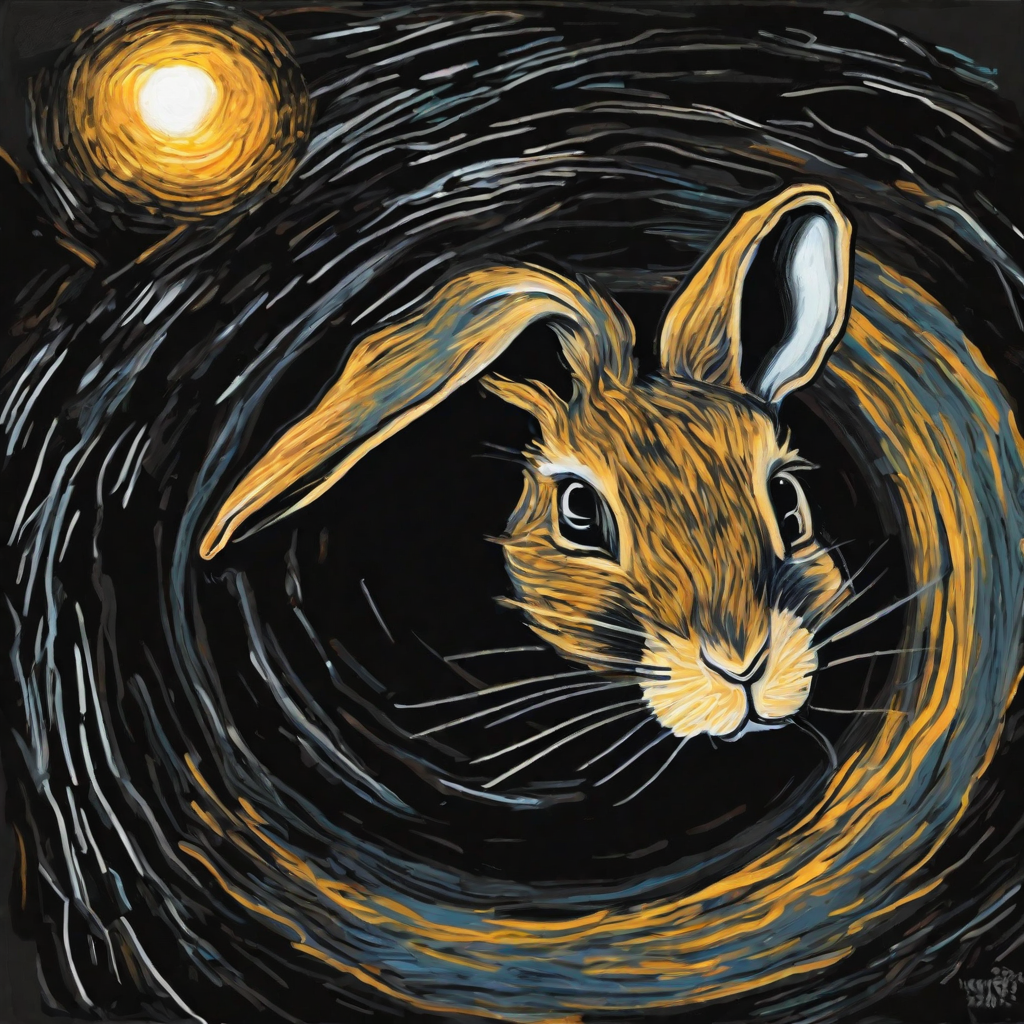
\includegraphics[width=0.6\textwidth]{fig/ch1/rabbit.png}
  \caption{时空穿越中的兔子}
  \label{fig:rabbit}
\end{figure}

\section{本文主要内容和组织结构}

本文的组织结构如下：

第一章，绪论。介绍超音速牛奶喷射和时间旅行的概率动力学研究的重要性和意义。

第二章，超音速牛奶喷射的流体动力学分析。

第三章，时间旅行的概率动力学模型。

第四章，超音速牛奶喷射与时间旅行的耦合分析。

第五章，总结与展望。
